\onecolumn
\begin{landscape}
\centering
\vspace*{\fill}
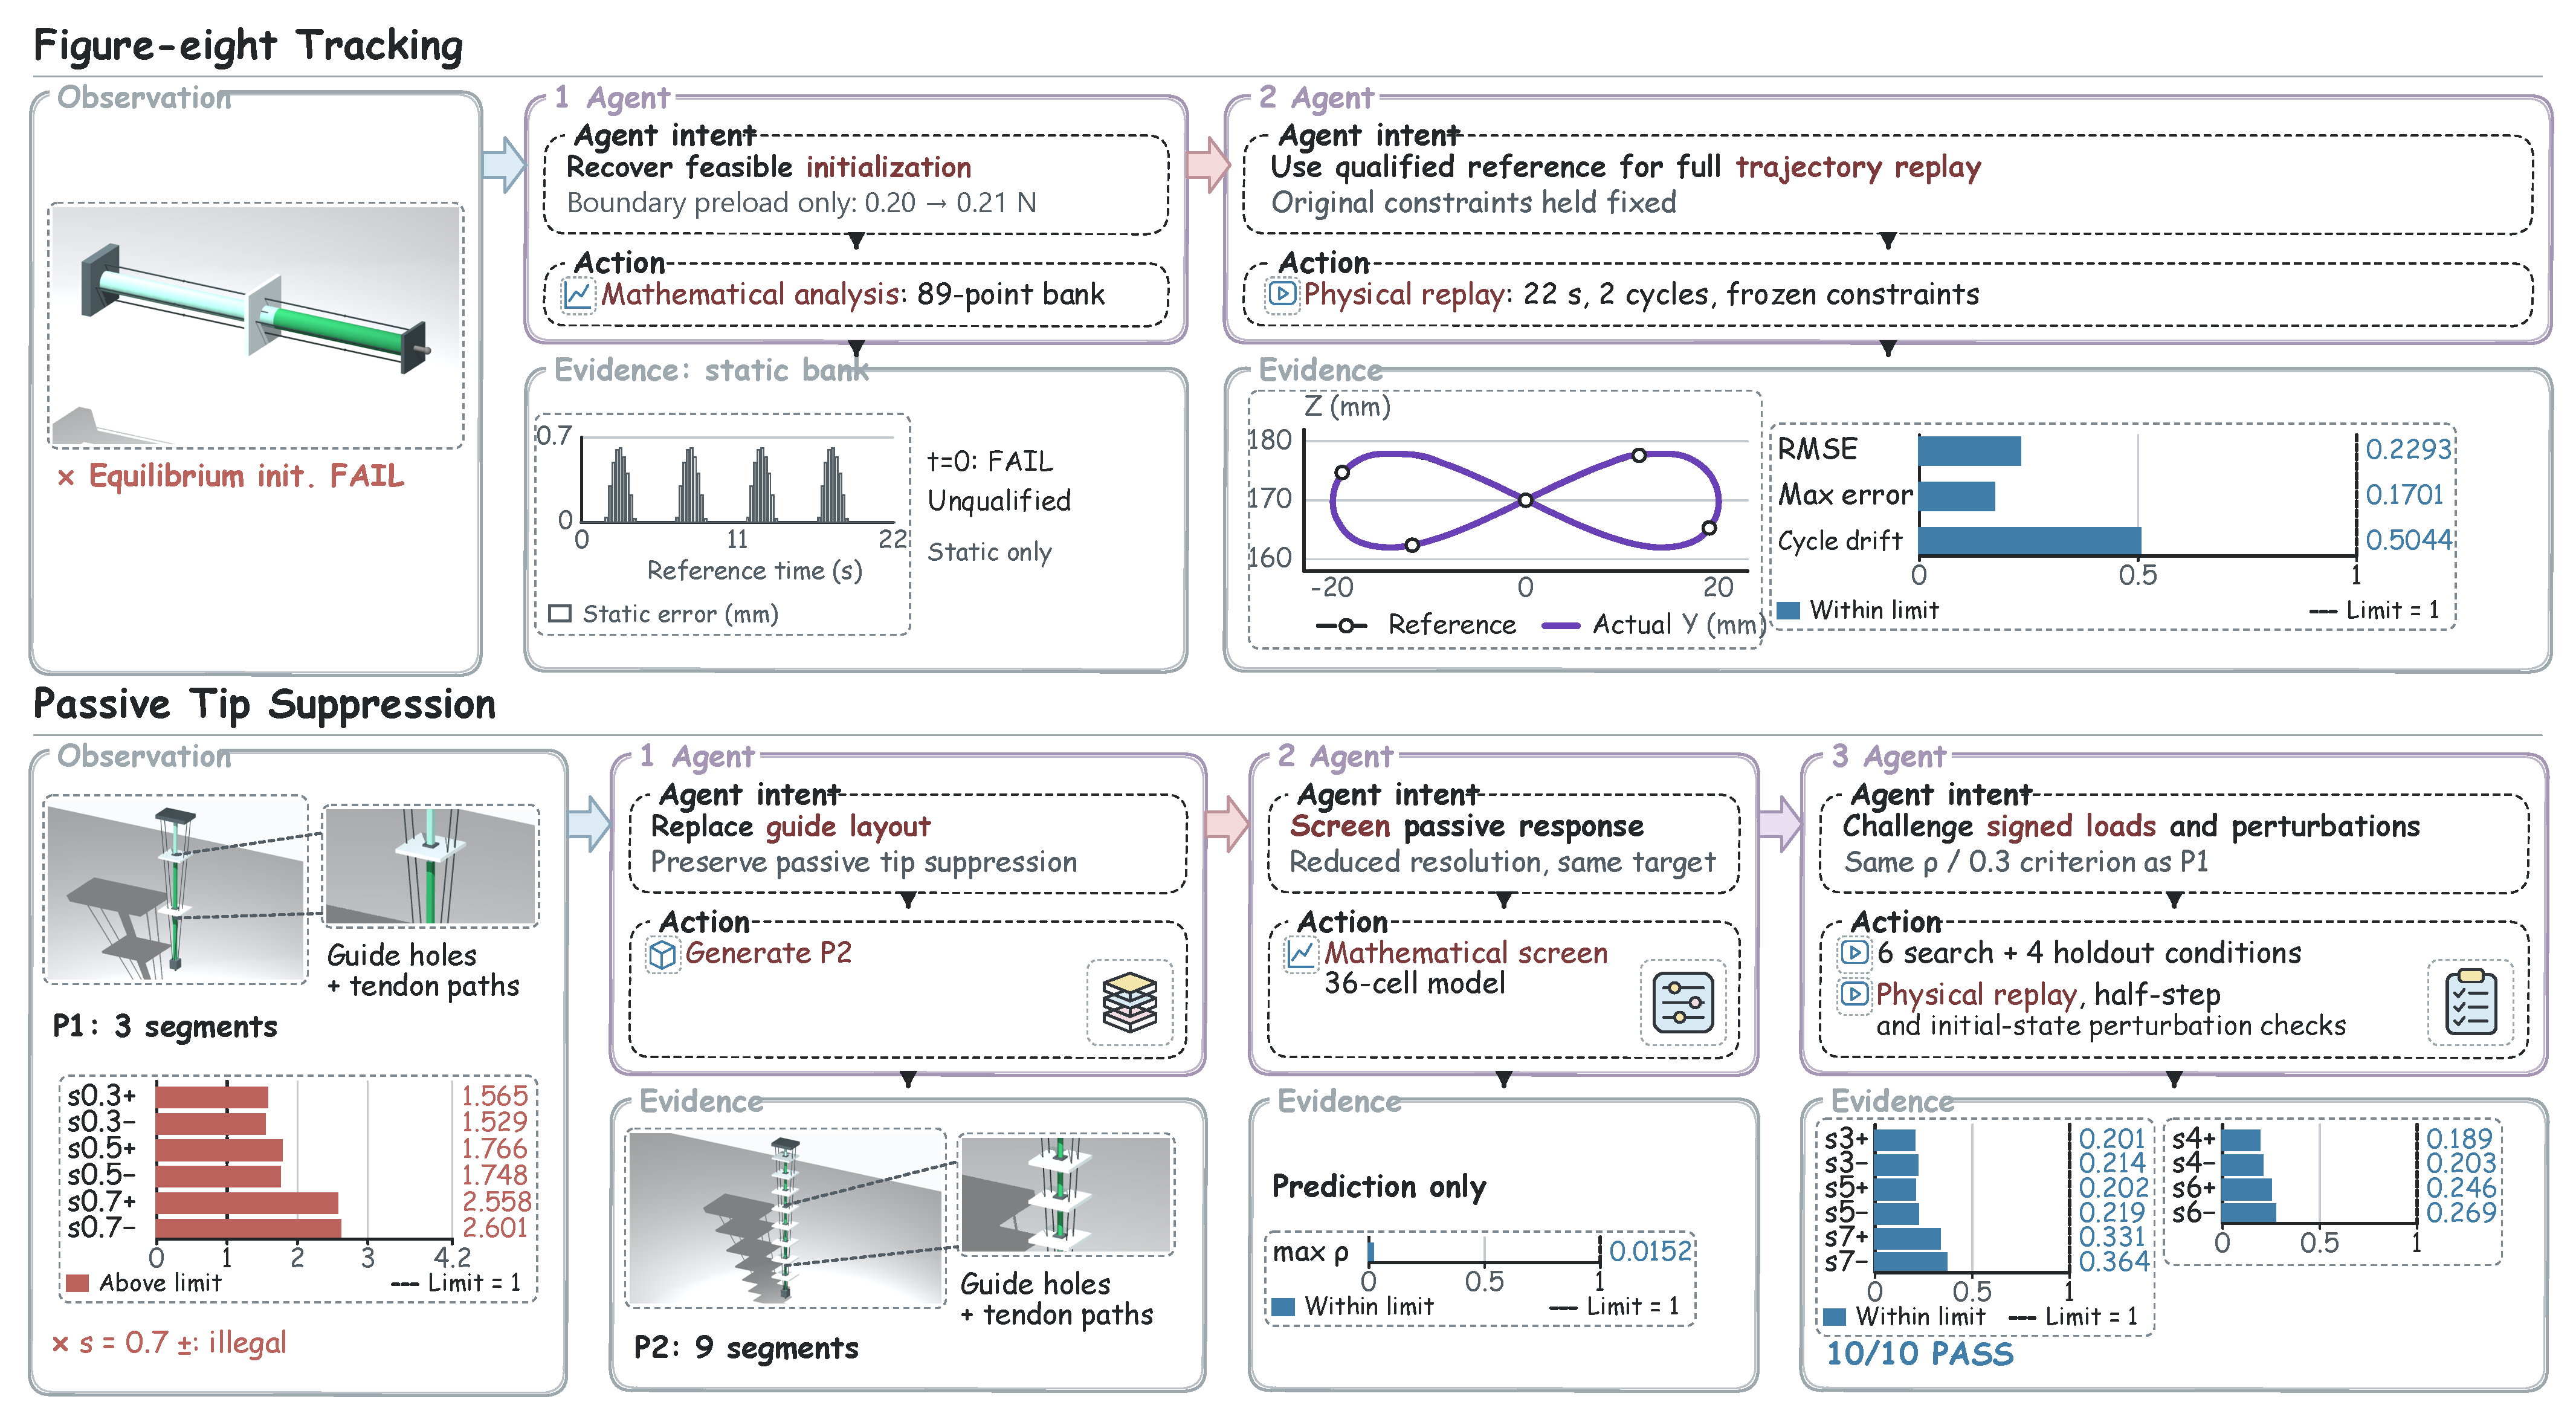
\includegraphics[width=\linewidth,height=0.84\textheight,keepaspectratio]{figures/fig03_agent_directed_research_a.pdf}\par
\landscapefigcaption{Agent-directed research process, part 1: T04 figure-eight tracking and PHS-2D passive tip suppression. The Main Agent converts observations into hypotheses, selects mathematical or physical investigations, and adapts subsequent actions.}
\label{fig:agent-directed-research}
\vspace*{\fill}
\end{landscape}
\begin{landscape}
\centering
\vspace*{\fill}
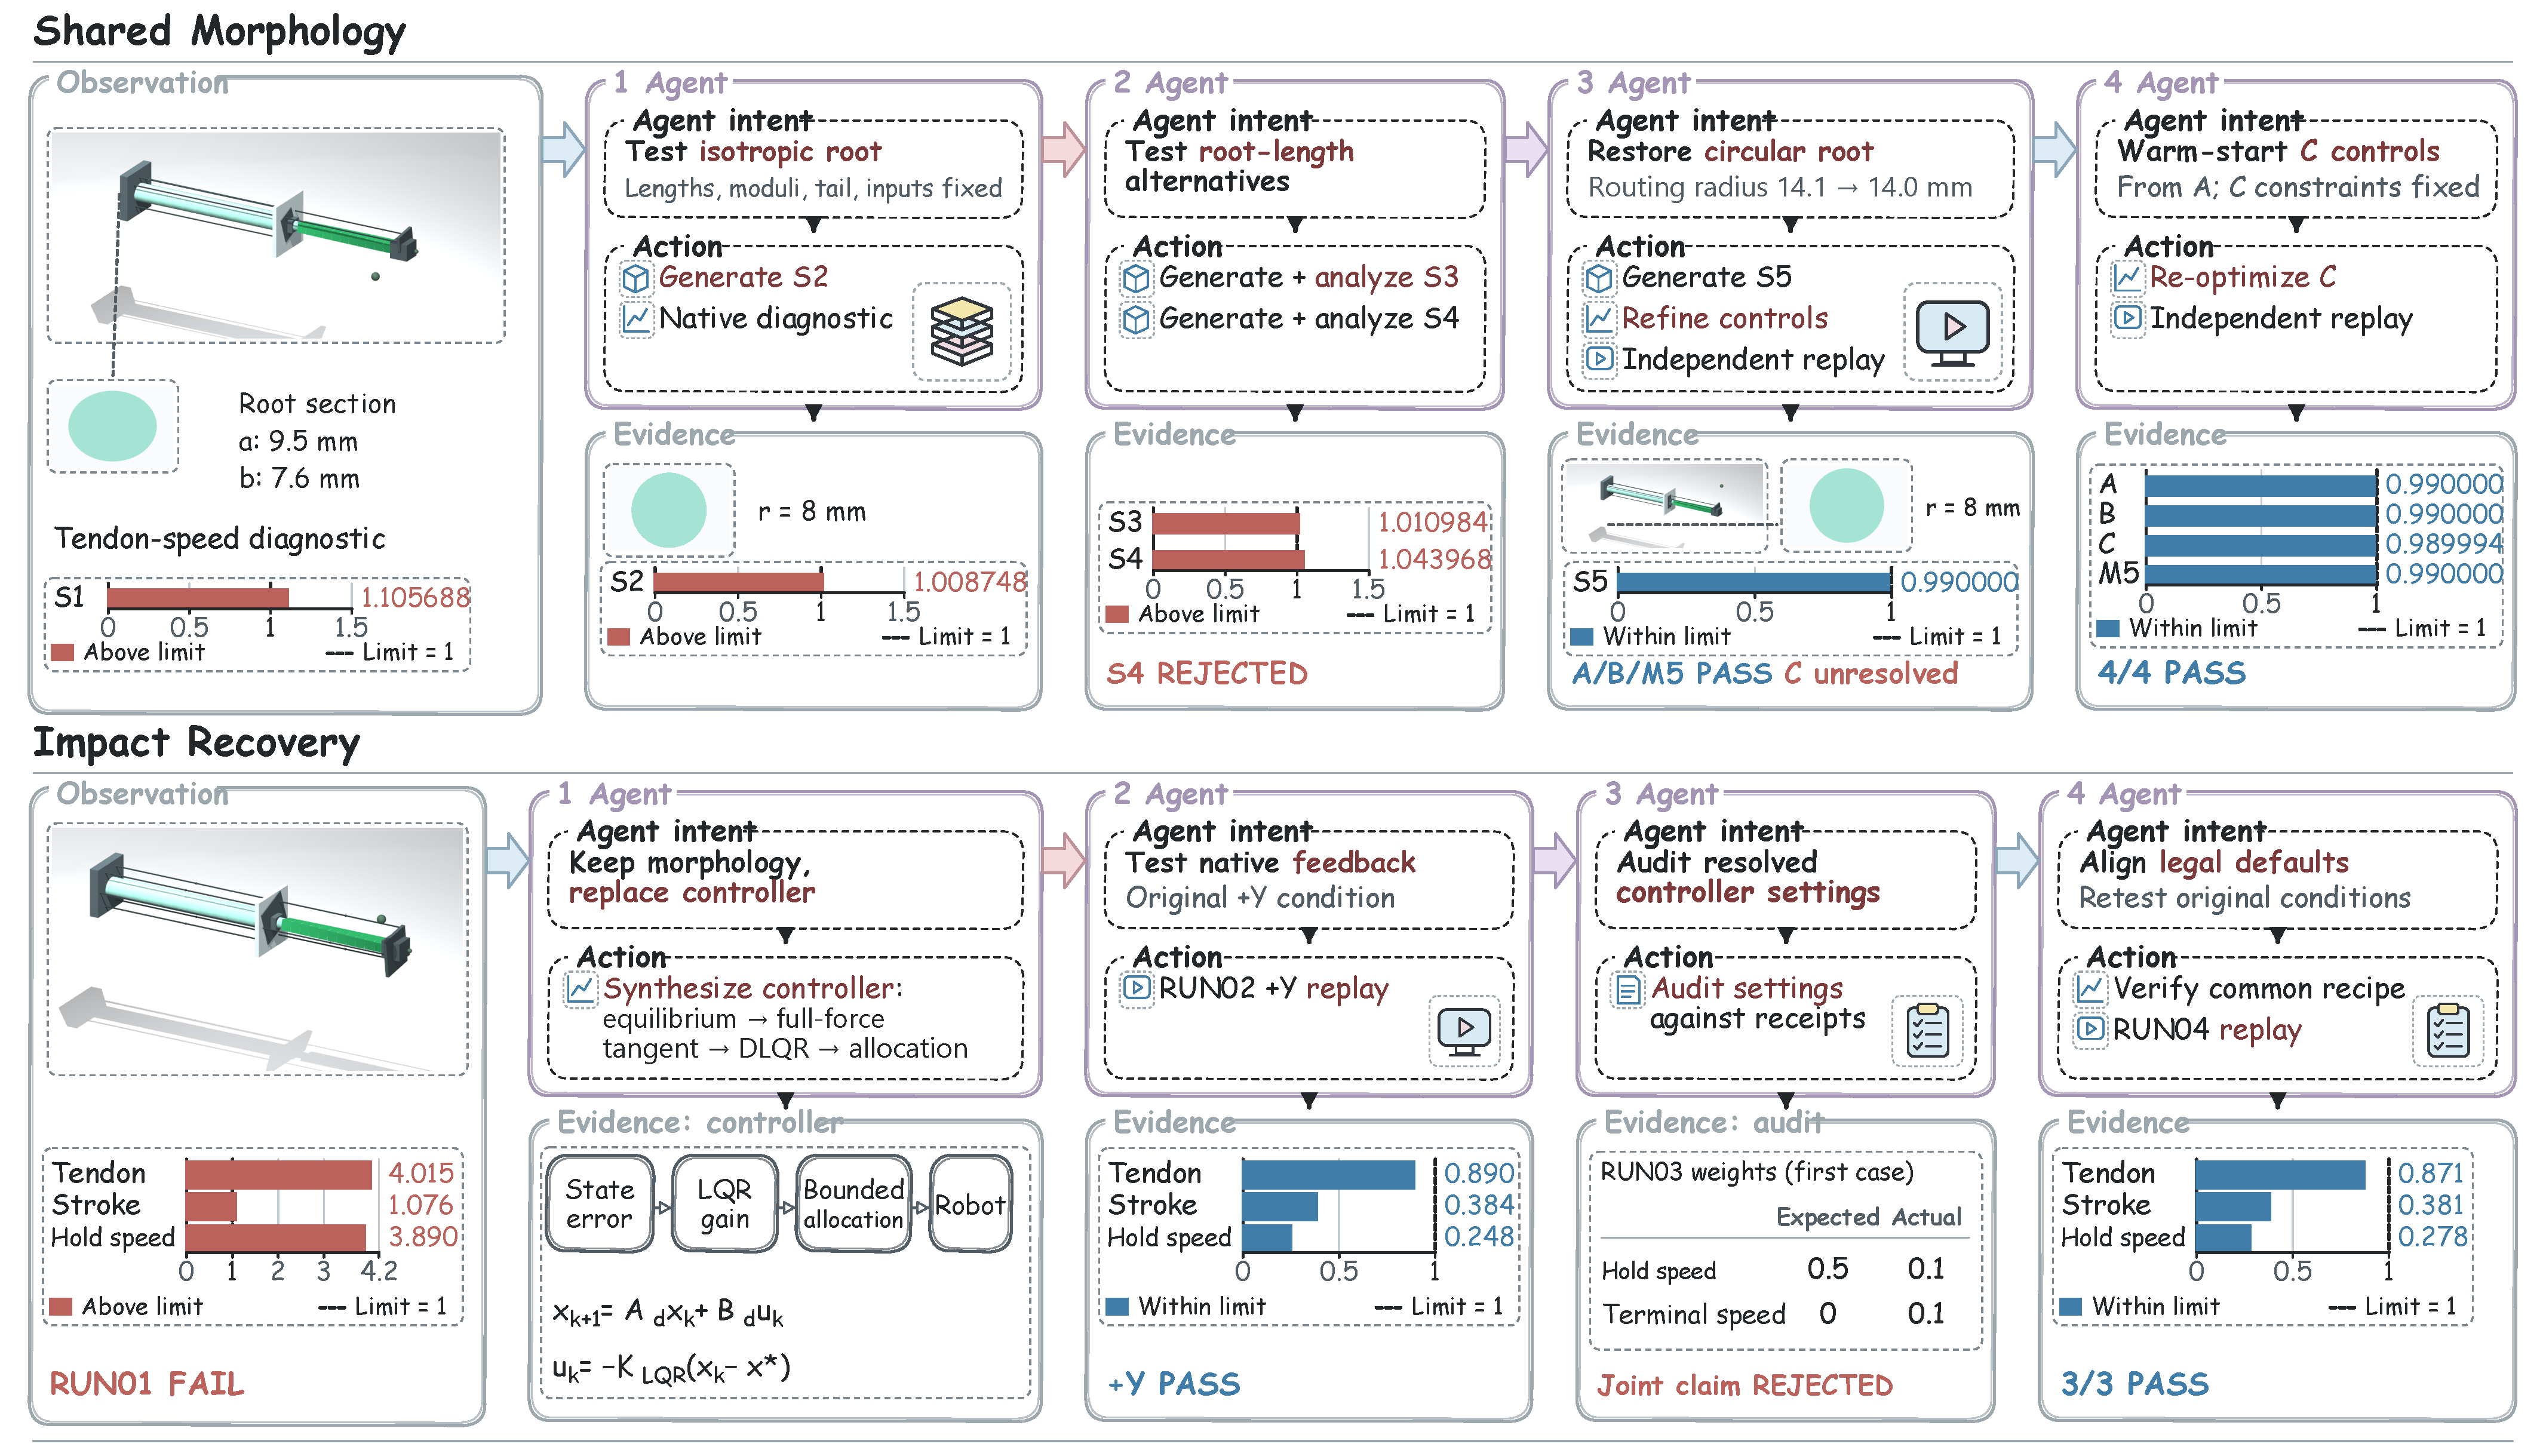
\includegraphics[width=\linewidth,height=0.84\textheight,keepaspectratio]{figures/fig03_agent_directed_research_b.pdf}\par
\addtocounter{figure}{-1}
\landscapefigcaption{Agent-directed research process, part 2 (continued): T07 shared morphology and T10 impact recovery. The cases illustrate selected decisions rather than a mandatory M0--M3 sequence.}
\vspace*{\fill}
\end{landscape}
\twocolumn
